%
% File naacl2019.tex
%
%% Based on the style files for ACL 2018 and NAACL 2018, which were
%% Based on the style files for ACL-2015, with some improvements
%%  taken from the NAACL-2016 style
%% Based on the style files for ACL-2014, which were, in turn,
%% based on ACL-2013, ACL-2012, ACL-2011, ACL-2010, ACL-IJCNLP-2009,
%% EACL-2009, IJCNLP-2008...
%% Based on the style files for EACL 2006 by
%%e.agirre@ehu.es or Sergi.Balari@uab.es
%% and that of ACL 08 by Joakim Nivre and Noah Smith

\documentclass[11pt,a4paper]{article}
\usepackage[hyperref]{naaclhlt2019}
\usepackage{times}
\usepackage{latexsym}
\usepackage{graphicx}

\usepackage{url}

\aclfinalcopy % Uncomment this line for the final submission
%\def\aclpaperid{***} %  Enter the acl Paper ID here

%\setlength\titlebox{5cm}
% You can expand the titlebox if you need extra space
% to show all the authors. Please do not make the titlebox
% smaller than 5cm (the original size); we will check this
% in the camera-ready version and ask you to change it back.

\newcommand\BibTeX{B{\sc ib}\TeX}

\title{Instructions for Dialogue Systems Final Project Report: Guess-What}

\author{Derek Acosta\\
  Georgetown University \\
  {\tt da606@georgetown.du} \\
Jiayue Wu \\
  Georgetown University \\
  {\tt jw1783@georgetown.edu} \\}

\date{}

\begin{document}
\maketitle
\begin{abstract}
  This is a report for the final project of dialogue system class. The project is a guess-what game, which means computer give out an image and let user guess the object in the image. In this report, we will talk about project's main tasks, how we tried to realized it, difficulties we had met and results we went out.
\end{abstract}

\section{Introduction}
As machine learning grows prominence venues for security are also becoming much more of an necessarily. ReCAPTCHA has serviced the world in protecting against spamming engines, DDOS attacks, and many other endeavors, but the question we were looking like is what if dialogue could be integrated into such a engine. Dialogue offers communication between parties and offering a security approach that relies on the exchange between two participants (AI and human). For the final project, we made a visual dialogue system using python2, which is a guess-what game. This type of application has motivations in security, games, and linguistics. By evaluating security we could collect how people are looking at photos or motion graphs and pursue to build up a model that offer basic interaction. The game approach factors in by having human answer questions that help unlock and move past a security wall. Lastly linguistic  fundamental are there that would allow for pictorial, descriptive longitudinal studies to be conducted online. The Basically, there are two plans. For plan A, we tried to make a guess-what game using LSTM model to encode word vectors and using MLP algorithm to train and predict results. For plan B, we tended to use Clarifai and wit.ai to process data, and work out a guess-what game.

\section{Task Description}

In this section, we will explain our main idea about the project. Basically, there are two plans. Both of the plans is a guess-what game based on image recognization.

\subsection{Plan A}
For plan A, we attempted to build a guess-what system based on existed dataset for this game. Rule for this game is as following: System will randomly give out an image, and get a crop with object in it. User can only see the image, and need to answer questions to system in order to guess what is in the crop. System will answer yes, no or N/A. After six terms, if user still can not determine what the object is, he will lose the game.

\subsection{Plan B}

For plan B, we tried to build a guess-what game based on clarifai and wit.ai. System is expected to give out a blurred image randomly. User ask question to guess what is in the image. System will answer the possibility of it's existence. If user get more than three objects in the image within six turns, he wins.

\section{Data Structure}
\label{sect:pdf}

In this section, we will introduce our data structure separately for two different plans.

\subsection{Plan A}
\label{ssec:layout}

For plan A, we use MS COCO dataset as the resource of images. We also use guess-what dataset for data training and prediction. In this case, we build our data structure according to these two datasets. There are three main classes, which is initial, image, qa and crop.

{\bf Initial}: This class on behalf of a task. It includes the task id, image object, qa object, crop object and timestamp. Timestamp is set to calculate the duration time of each task, so that we can take it as one of the aspects to evaluate the system.

{\bf Image}: This class is used to store image information, including image id width, height and url. Url is address of the image from MS COCO dataset. Something important is that images which are selected into this dataset all have various objects in them. So the system can randomly choose one object from them and give out the game task.

{\bf Qa}: This class is used to store questions from users and answers from system. The original questions and answers from guess-what datatable are collected from manual answers. The builders of guess-what datatable employed people and make each two of them as a pair. Each pair of employees have questions and answers with each other according to a specific object in the image they are given. Builders stored their conversation and used them in guess-what datatable.

{\bf Crop}: This class is used to store crop information. Information includes crop id, category id, category, bbox and segment. Category is the label of crop, in other words, it is the answer user need to guess. Bbox stores the positions of crop's four corners.

\begin{table}
\centering
\begin{tabular}{|l|l|}
\hline
{\bf Initial} & {\bf }\\\hline
\verb|id| & {int} \\
\verb|image| & {Image} \\
\verb|qa| & {Qa} \\
\verb|crop| & {Crop} \\
\verb|timestamp| & {int} \\\hline
\end{tabular} &
\begin{tabular}{|l|l|}
\hline
{\bf Image} & {\bf}\\\hline
\verb|id| & {int} \\
\verb|width| & {int} \\
\verb|height| & {int} \\
\verb|url| & {str} \\\hline
\end{tabular}
\begin{tabular}{|l|l|}
\hline
{\bf Qa} & {\bf }\\\hline
\verb|id| & {int} \\
\verb|answer| & {Either 'YES', 'No' or 'N/A'} \\
\verb|question| & {str} \\\hline
\end{tabular} &
\begin{tabular}{|l|l|}
\hline
{\bf Crop} & {\bf}\\\hline
\verb|id| & {int} \\
\verb|category_id| & {int} \\
\verb|category| & {str} \\
\verb|bbox| & {x, y, width, height} \\
\verb|segment| & {polygon} \\\hline
\end{tabular}
\caption{Data structure for plan A.}\label{tab:accents}
\end{table}

\subsection{Plan B}

In plan B, the most important elements are concept list, user input list, keyword list and keyword position list. Concept list used to store image concepts responsed by Clarifai. User input list used to process user inputs. keyword list stores keywords get from user input list. keyword position records the positions of keywords in concept list. 


\section{Tools}
\label{ssec:first}

In this section, we will discuss tools we used to realize our project. 


\subsection{Plan A}

When it comes to plan A, three most important tools are Tensorflow, Pillow and Json.
\begin{itemize}
\item {\bf Tensorflow}: It is an open source library which we used to encode word vectors through LSTM module and decode from softmax layer.
\item {\bf Pillow}: This library is imported to do some image operations. For example, we use it to show images, crop it according to bbox area.
\item {\bf Json} This library is used to import guess-what dataset.
\end{itemize}


\subsection{Plan B}

For plan B, the most core tools we used are Clarifai and Wit.ai.
\begin{itemize}
\item {\bf Clarifai}: This is a vision AI, which has a variety of different models. For example, color, apparel, food. Users import images, and by using different models, they can get the response including a lot of information about the image in the specific model area. The information users get includes concept id, concept name, concept value.
\item {\bf Wit.ai}: This is a AI which can gets what user said and get useful information from input sentences, including date, name, position, etc. Users can also define their own kind of keywords.
\end{itemize}

\section{Process}

In this section, we will discuss more about how we build our project. For plan A, the process includes how we train data and get the predict data. For plan B, the process is mainly how we get the concepts of the image, how we get keyword's from users' input and the way we connect the concepts and keywords together.


\subsection{Plan A}
\label{ssec:accessibility}
As has said before, we imported questions and answers from guess-what dataset. Each object has about 8 pairs of questions and answers. We attempted to train these human conversation, and predict the answer of new inputs. 

Before we introduce Qa class into train model, we did some preparations. Firstly, we split the sentences into words.

{\bf Reverse}: We discovered that the word at the ending part of a sentence are more likely to be important. For instance, when user input "ls it a bear?", the keyword we want to capture is "bear", and it appears at the end of the sentence. For this reason, we first had a reverse operation on sentences both for train and predict.

{\bf Enhance}: For the reason that eight pairs of Qa for each object is too little for training, we enhanced data by shuffled words in question to get new samples.

{\bf Shuffle}: Besides shuffled the components in questions, we also shuffled the order of questions, so that we can ensure train model get random sample, and in this way to improve the quality of training.

After embedding each word, the sentence vector entered the LSTM layer, where the standard LSTM is used, and then a vector of n hidden LSTM neural units obtained through a time series is obtained. After passing through the mean pooling layer, a vector h can be obtained, and then Following a Softmax layer, a class distribution probability vector is obtained, and the category with the highest probability value is taken as the final prediction result.


\subsection{Plan B}
\label{ssec:accessibility}

Building this system involved many moving part stemming from Wit.ai, Clarifai and porting to a flask, node.js server. The process here consisting of delegating the aforementioned services to behave cohesively in our architecture. The management consisted of using Wit.ai for NLU support and requesting (cURLing) responses from it to post and get results through user response and our own normalized and scrubbed data. 
When plan A fell through, we had to generate text samples that were solely image specific but had a myriad of details. We decided to do a description questionnaire game that utilized Clarifai's image tagging capability and making question based on the systems classification. By using this approach we could gather information on the image and in real-time render out questions related to the users. 


\section{Difficulty}

In this part, we will discuss difficulties we met during the process we build both plan A and plan B. Because of the problems we found, we finally decided to give up plan A.

\subsection{Plan A}
\label{sec:length}

There were two main problems that obstructed us in plan A.

Firstly, we found that data from guess-what dataset didn’t relate ‘qa’ to ‘crop’. There are a lot of crops
in one image, but only one set of Qa that is related to one of the crop. Moreover, the dataset doesn't show any relationship between this set of Qa and it's crop, which means even we developers need to determine the target crop by ourselves.

Besides, the result we get from the model is always 'N/A', which we can not fix yet.


\subsection{Plan B}
\label{sec:length}

There were several obstacles in are way when pursuing Plan B. Generating Wit.ai tags and intent related to stochastic visuals and images become difficult to manage and often time we wanted to default to using regex or difflib library to compute similarity between the correct answer and the user’s response. In sticking with Wit.ai and feeding it more data eventually out-weighted in both effort and confidence as it began performing much better. Additionally setting up the code to port to a web server has rather difficult because of the system we were trying to optimize for did not necessarily lend themselves to terminal clients. 

\begin{figure}
    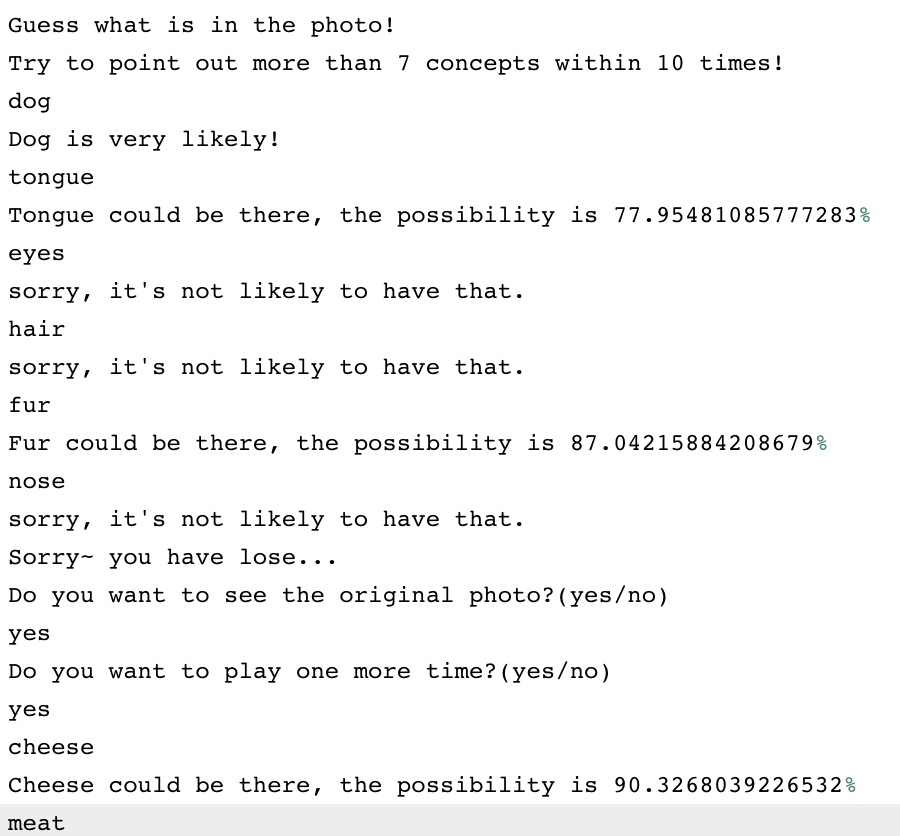
\includegraphics[width=\linewidth]{dialex.jpg}
    \caption{Dialogue from an evaluation session}
\end{figure}
\section*{Evaluation}

Evaluation was conducted using informal surveys of family and friends adding to roughly 10 people. These participants are technically adapt in using computers, browsers, and are not visually impaired. All the participants played the game twice. We pushed for them to be as open with their phrasing as possible, but even with that subjects understand the potential of the system, but found that it difficult to know what the system was capable of doing. As figure 1 demonstrates, the system is out-rightly prepared for modest answer. The aspect of asking questions in a system like this might throws someone off what they were given a guide of what was available to them. 
The user in figure 1 noted the ambiguity in looking know what exactly to look for. In first couple of utterances we saw that subject were inclined to use certain kind of phrases that would normally register as natural in a human to human conversation. What we found is that system had a hard time recognizing certain intent in utterances that began with "is this." This utterance seem to come out of some preconceived ideas of how communicating my dialogue system goes. Some issue we experienced in was that for some words when passed them through a porter would lose some of its context was we tried to filters and pass the responses with variable spelling. There were some cases that the user knew the answer but had to give up because the phrasing of the answer and spelling were a bit off. Once we evaluated the responses by humans we cataloged them into Wit.ai to try and heighten our precision and accuracy scores. \\

\section*{Improvement}

Following the feedback from the evaluation, we shifted our development from implementing features to correcting certain problem area. The first couple we focused on pertained to using the Porter stemmer which we used to normalize a good portion of our data. Tandem to this we made edits to Wit.ai and augmented our options list in python to accommodate  for more variable and accommodate for more variable responses. In the process of doing that we were notice that, participate wanted options for when they were frustrated to often skip the photo on command or for the system to understand that they were irked. Often times, participates would use keywords like "idk" or "not sure" to spelled out confusion but the system could not properly index this intents accurately. While Wit.ai is great at performing task its already seen, it does poorly to learn from utterance it has not been directly trained on. For utterances it has not yet encountered, performance remained somewhat troublesome. With more training this could solve many of these issues by adding in from data. Other difficulties we had pertain to how Wit classified sentences without much context behind them meaning its more adapt at deciphering long sentence other smaller ones. Given more time to fiddle with the system we would have tried a Wizard of Oz approach to gauge more naturalized occurrences that preferably were not one word responses. 

\section*{Discussion}
The domains that these games could be tailored can service both security and educational functions. Having users respond to question can aid in the dialogue sphere by aggregating dialogue specific to visuals. This can improve in understanding where users are directing their attention and have features of these visuals are the most pertinent. Dialogue can service these domains by adding a level of quizzical-ness that can both make it harder for system to mask as human but also act in a way that is much more fluid and context dependent. 

\section*{Conclusion}
As it stand, that functionality the system has is not barred by much other than the influx of images. For a more cohesive experiences the application best lends itself to the web and offers much more flexibility and usability as a traditional reCAPTCHA system would. If nothing else, the project has allowed us to experience different ranges of research and image recognition and the pitfalls within conversation. Like many things more time would grant us the option to for more research, feedback reception, and proper presentation. 

\appendix


\section{Supplemental Material}
\label{sec:supplemental}
De Vries, H., Strub, F., Chandar, S., Pietquin, O., Larochelle, H., & Courville, A. C. (2017, July). GuessWhat?! Visual object discovery through multi-modal dialogue. 


Das, A., Kottur, S., Gupta, K., Singh, A., Yadav, D., Moura, J. M., ... & Batra, D. (2017, July). Visual dialog. In Proceedings of the IEEE Conference on Computer Vision and Pattern Recognition(Vol. 2).


Mostafazadeh, N., Brockett, C., Dolan, B., Galley, M., Gao, J., Spithourakis, G. P., & Vanderwende, L. (2017). Image-grounded conversations: Multimodal context for natural question and response generation. In Proc. of IJCNLP.

\end{document}
